\documentclass[11pt]{article}

    \usepackage[breakable]{tcolorbox}
    \usepackage{parskip} % Stop auto-indenting (to mimic markdown behaviour)
    

    % Basic figure setup, for now with no caption control since it's done
    % automatically by Pandoc (which extracts ![](path) syntax from Markdown).
    \usepackage{graphicx}
    % Keep aspect ratio if custom image width or height is specified
    \setkeys{Gin}{keepaspectratio}
    % Maintain compatibility with old templates. Remove in nbconvert 6.0
    \let\Oldincludegraphics\includegraphics
    % Ensure that by default, figures have no caption (until we provide a
    % proper Figure object with a Caption API and a way to capture that
    % in the conversion process - todo).
    \usepackage{caption}
    \DeclareCaptionFormat{nocaption}{}
    \captionsetup{format=nocaption,aboveskip=0pt,belowskip=0pt}

    \usepackage{float}
    \floatplacement{figure}{H} % forces figures to be placed at the correct location
    \usepackage{xcolor} % Allow colors to be defined
    \usepackage{enumerate} % Needed for markdown enumerations to work
    \usepackage{geometry} % Used to adjust the document margins
    \usepackage{amsmath} % Equations
    \usepackage{amssymb} % Equations
    \usepackage{textcomp} % defines textquotesingle
    % Hack from http://tex.stackexchange.com/a/47451/13684:
    \AtBeginDocument{%
        \def\PYZsq{\textquotesingle}% Upright quotes in Pygmentized code
    }
    \usepackage{upquote} % Upright quotes for verbatim code
    \usepackage{eurosym} % defines \euro

    \usepackage{iftex}
    \ifPDFTeX
        \usepackage[T1]{fontenc}
        \IfFileExists{alphabeta.sty}{
              \usepackage{alphabeta}
          }{
              \usepackage[mathletters]{ucs}
              \usepackage[utf8x]{inputenc}
          }
    \else
        \usepackage{fontspec}
        \usepackage{unicode-math}
    \fi

    \usepackage{fancyvrb} % verbatim replacement that allows latex
    \usepackage{grffile} % extends the file name processing of package graphics
                         % to support a larger range
    \makeatletter % fix for old versions of grffile with XeLaTeX
    \@ifpackagelater{grffile}{2019/11/01}
    {
      % Do nothing on new versions
    }
    {
      \def\Gread@@xetex#1{%
        \IfFileExists{"\Gin@base".bb}%
        {\Gread@eps{\Gin@base.bb}}%
        {\Gread@@xetex@aux#1}%
      }
    }
    \makeatother
    \usepackage[Export]{adjustbox} % Used to constrain images to a maximum size
    \adjustboxset{max size={0.9\linewidth}{0.9\paperheight}}

    % The hyperref package gives us a pdf with properly built
    % internal navigation ('pdf bookmarks' for the table of contents,
    % internal cross-reference links, web links for URLs, etc.)
    \usepackage{hyperref}
    % The default LaTeX title has an obnoxious amount of whitespace. By default,
    % titling removes some of it. It also provides customization options.
    \usepackage{titling}
    \usepackage{longtable} % longtable support required by pandoc >1.10
    \usepackage{booktabs}  % table support for pandoc > 1.12.2
    \usepackage{array}     % table support for pandoc >= 2.11.3
    \usepackage{calc}      % table minipage width calculation for pandoc >= 2.11.1
    \usepackage[inline]{enumitem} % IRkernel/repr support (it uses the enumerate* environment)
    \usepackage[normalem]{ulem} % ulem is needed to support strikethroughs (\sout)
                                % normalem makes italics be italics, not underlines
    \usepackage{soul}      % strikethrough (\st) support for pandoc >= 3.0.0
    \usepackage{mathrsfs}
    

    
    % Colors for the hyperref package
    \definecolor{urlcolor}{rgb}{0,.145,.698}
    \definecolor{linkcolor}{rgb}{.71,0.21,0.01}
    \definecolor{citecolor}{rgb}{.12,.54,.11}

    % ANSI colors
    \definecolor{ansi-black}{HTML}{3E424D}
    \definecolor{ansi-black-intense}{HTML}{282C36}
    \definecolor{ansi-red}{HTML}{E75C58}
    \definecolor{ansi-red-intense}{HTML}{B22B31}
    \definecolor{ansi-green}{HTML}{00A250}
    \definecolor{ansi-green-intense}{HTML}{007427}
    \definecolor{ansi-yellow}{HTML}{DDB62B}
    \definecolor{ansi-yellow-intense}{HTML}{B27D12}
    \definecolor{ansi-blue}{HTML}{208FFB}
    \definecolor{ansi-blue-intense}{HTML}{0065CA}
    \definecolor{ansi-magenta}{HTML}{D160C4}
    \definecolor{ansi-magenta-intense}{HTML}{A03196}
    \definecolor{ansi-cyan}{HTML}{60C6C8}
    \definecolor{ansi-cyan-intense}{HTML}{258F8F}
    \definecolor{ansi-white}{HTML}{C5C1B4}
    \definecolor{ansi-white-intense}{HTML}{A1A6B2}
    \definecolor{ansi-default-inverse-fg}{HTML}{FFFFFF}
    \definecolor{ansi-default-inverse-bg}{HTML}{000000}

    % common color for the border for error outputs.
    \definecolor{outerrorbackground}{HTML}{FFDFDF}

    % commands and environments needed by pandoc snippets
    % extracted from the output of `pandoc -s`
    \providecommand{\tightlist}{%
      \setlength{\itemsep}{0pt}\setlength{\parskip}{0pt}}
    \DefineVerbatimEnvironment{Highlighting}{Verbatim}{commandchars=\\\{\}}
    % Add ',fontsize=\small' for more characters per line
    \newenvironment{Shaded}{}{}
    \newcommand{\KeywordTok}[1]{\textcolor[rgb]{0.00,0.44,0.13}{\textbf{{#1}}}}
    \newcommand{\DataTypeTok}[1]{\textcolor[rgb]{0.56,0.13,0.00}{{#1}}}
    \newcommand{\DecValTok}[1]{\textcolor[rgb]{0.25,0.63,0.44}{{#1}}}
    \newcommand{\BaseNTok}[1]{\textcolor[rgb]{0.25,0.63,0.44}{{#1}}}
    \newcommand{\FloatTok}[1]{\textcolor[rgb]{0.25,0.63,0.44}{{#1}}}
    \newcommand{\CharTok}[1]{\textcolor[rgb]{0.25,0.44,0.63}{{#1}}}
    \newcommand{\StringTok}[1]{\textcolor[rgb]{0.25,0.44,0.63}{{#1}}}
    \newcommand{\CommentTok}[1]{\textcolor[rgb]{0.38,0.63,0.69}{\textit{{#1}}}}
    \newcommand{\OtherTok}[1]{\textcolor[rgb]{0.00,0.44,0.13}{{#1}}}
    \newcommand{\AlertTok}[1]{\textcolor[rgb]{1.00,0.00,0.00}{\textbf{{#1}}}}
    \newcommand{\FunctionTok}[1]{\textcolor[rgb]{0.02,0.16,0.49}{{#1}}}
    \newcommand{\RegionMarkerTok}[1]{{#1}}
    \newcommand{\ErrorTok}[1]{\textcolor[rgb]{1.00,0.00,0.00}{\textbf{{#1}}}}
    \newcommand{\NormalTok}[1]{{#1}}

    % Additional commands for more recent versions of Pandoc
    \newcommand{\ConstantTok}[1]{\textcolor[rgb]{0.53,0.00,0.00}{{#1}}}
    \newcommand{\SpecialCharTok}[1]{\textcolor[rgb]{0.25,0.44,0.63}{{#1}}}
    \newcommand{\VerbatimStringTok}[1]{\textcolor[rgb]{0.25,0.44,0.63}{{#1}}}
    \newcommand{\SpecialStringTok}[1]{\textcolor[rgb]{0.73,0.40,0.53}{{#1}}}
    \newcommand{\ImportTok}[1]{{#1}}
    \newcommand{\DocumentationTok}[1]{\textcolor[rgb]{0.73,0.13,0.13}{\textit{{#1}}}}
    \newcommand{\AnnotationTok}[1]{\textcolor[rgb]{0.38,0.63,0.69}{\textbf{\textit{{#1}}}}}
    \newcommand{\CommentVarTok}[1]{\textcolor[rgb]{0.38,0.63,0.69}{\textbf{\textit{{#1}}}}}
    \newcommand{\VariableTok}[1]{\textcolor[rgb]{0.10,0.09,0.49}{{#1}}}
    \newcommand{\ControlFlowTok}[1]{\textcolor[rgb]{0.00,0.44,0.13}{\textbf{{#1}}}}
    \newcommand{\OperatorTok}[1]{\textcolor[rgb]{0.40,0.40,0.40}{{#1}}}
    \newcommand{\BuiltInTok}[1]{{#1}}
    \newcommand{\ExtensionTok}[1]{{#1}}
    \newcommand{\PreprocessorTok}[1]{\textcolor[rgb]{0.74,0.48,0.00}{{#1}}}
    \newcommand{\AttributeTok}[1]{\textcolor[rgb]{0.49,0.56,0.16}{{#1}}}
    \newcommand{\InformationTok}[1]{\textcolor[rgb]{0.38,0.63,0.69}{\textbf{\textit{{#1}}}}}
    \newcommand{\WarningTok}[1]{\textcolor[rgb]{0.38,0.63,0.69}{\textbf{\textit{{#1}}}}}
    \makeatletter
    \newsavebox\pandoc@box
    \newcommand*\pandocbounded[1]{%
      \sbox\pandoc@box{#1}%
      % scaling factors for width and height
      \Gscale@div\@tempa\textheight{\dimexpr\ht\pandoc@box+\dp\pandoc@box\relax}%
      \Gscale@div\@tempb\linewidth{\wd\pandoc@box}%
      % select the smaller of both
      \ifdim\@tempb\p@<\@tempa\p@
        \let\@tempa\@tempb
      \fi
      % scaling accordingly (\@tempa < 1)
      \ifdim\@tempa\p@<\p@
        \scalebox{\@tempa}{\usebox\pandoc@box}%
      % scaling not needed, use as it is
      \else
        \usebox{\pandoc@box}%
      \fi
    }
    \makeatother

    % Define a nice break command that doesn't care if a line doesn't already
    % exist.
    \def\br{\hspace*{\fill} \\* }
    % Math Jax compatibility definitions
    \def\gt{>}
    \def\lt{<}
    \let\Oldtex\TeX
    \let\Oldlatex\LaTeX
    \renewcommand{\TeX}{\textrm{\Oldtex}}
    \renewcommand{\LaTeX}{\textrm{\Oldlatex}}
    % Document parameters
    % Document title
    \title{11\_notes}
    
    
    
    
    
    
    
% Pygments definitions
\makeatletter
\def\PY@reset{\let\PY@it=\relax \let\PY@bf=\relax%
    \let\PY@ul=\relax \let\PY@tc=\relax%
    \let\PY@bc=\relax \let\PY@ff=\relax}
\def\PY@tok#1{\csname PY@tok@#1\endcsname}
\def\PY@toks#1+{\ifx\relax#1\empty\else%
    \PY@tok{#1}\expandafter\PY@toks\fi}
\def\PY@do#1{\PY@bc{\PY@tc{\PY@ul{%
    \PY@it{\PY@bf{\PY@ff{#1}}}}}}}
\def\PY#1#2{\PY@reset\PY@toks#1+\relax+\PY@do{#2}}

\@namedef{PY@tok@w}{\def\PY@tc##1{\textcolor[rgb]{0.73,0.73,0.73}{##1}}}
\@namedef{PY@tok@c}{\let\PY@it=\textit\def\PY@tc##1{\textcolor[rgb]{0.24,0.48,0.48}{##1}}}
\@namedef{PY@tok@cp}{\def\PY@tc##1{\textcolor[rgb]{0.61,0.40,0.00}{##1}}}
\@namedef{PY@tok@k}{\let\PY@bf=\textbf\def\PY@tc##1{\textcolor[rgb]{0.00,0.50,0.00}{##1}}}
\@namedef{PY@tok@kp}{\def\PY@tc##1{\textcolor[rgb]{0.00,0.50,0.00}{##1}}}
\@namedef{PY@tok@kt}{\def\PY@tc##1{\textcolor[rgb]{0.69,0.00,0.25}{##1}}}
\@namedef{PY@tok@o}{\def\PY@tc##1{\textcolor[rgb]{0.40,0.40,0.40}{##1}}}
\@namedef{PY@tok@ow}{\let\PY@bf=\textbf\def\PY@tc##1{\textcolor[rgb]{0.67,0.13,1.00}{##1}}}
\@namedef{PY@tok@nb}{\def\PY@tc##1{\textcolor[rgb]{0.00,0.50,0.00}{##1}}}
\@namedef{PY@tok@nf}{\def\PY@tc##1{\textcolor[rgb]{0.00,0.00,1.00}{##1}}}
\@namedef{PY@tok@nc}{\let\PY@bf=\textbf\def\PY@tc##1{\textcolor[rgb]{0.00,0.00,1.00}{##1}}}
\@namedef{PY@tok@nn}{\let\PY@bf=\textbf\def\PY@tc##1{\textcolor[rgb]{0.00,0.00,1.00}{##1}}}
\@namedef{PY@tok@ne}{\let\PY@bf=\textbf\def\PY@tc##1{\textcolor[rgb]{0.80,0.25,0.22}{##1}}}
\@namedef{PY@tok@nv}{\def\PY@tc##1{\textcolor[rgb]{0.10,0.09,0.49}{##1}}}
\@namedef{PY@tok@no}{\def\PY@tc##1{\textcolor[rgb]{0.53,0.00,0.00}{##1}}}
\@namedef{PY@tok@nl}{\def\PY@tc##1{\textcolor[rgb]{0.46,0.46,0.00}{##1}}}
\@namedef{PY@tok@ni}{\let\PY@bf=\textbf\def\PY@tc##1{\textcolor[rgb]{0.44,0.44,0.44}{##1}}}
\@namedef{PY@tok@na}{\def\PY@tc##1{\textcolor[rgb]{0.41,0.47,0.13}{##1}}}
\@namedef{PY@tok@nt}{\let\PY@bf=\textbf\def\PY@tc##1{\textcolor[rgb]{0.00,0.50,0.00}{##1}}}
\@namedef{PY@tok@nd}{\def\PY@tc##1{\textcolor[rgb]{0.67,0.13,1.00}{##1}}}
\@namedef{PY@tok@s}{\def\PY@tc##1{\textcolor[rgb]{0.73,0.13,0.13}{##1}}}
\@namedef{PY@tok@sd}{\let\PY@it=\textit\def\PY@tc##1{\textcolor[rgb]{0.73,0.13,0.13}{##1}}}
\@namedef{PY@tok@si}{\let\PY@bf=\textbf\def\PY@tc##1{\textcolor[rgb]{0.64,0.35,0.47}{##1}}}
\@namedef{PY@tok@se}{\let\PY@bf=\textbf\def\PY@tc##1{\textcolor[rgb]{0.67,0.36,0.12}{##1}}}
\@namedef{PY@tok@sr}{\def\PY@tc##1{\textcolor[rgb]{0.64,0.35,0.47}{##1}}}
\@namedef{PY@tok@ss}{\def\PY@tc##1{\textcolor[rgb]{0.10,0.09,0.49}{##1}}}
\@namedef{PY@tok@sx}{\def\PY@tc##1{\textcolor[rgb]{0.00,0.50,0.00}{##1}}}
\@namedef{PY@tok@m}{\def\PY@tc##1{\textcolor[rgb]{0.40,0.40,0.40}{##1}}}
\@namedef{PY@tok@gh}{\let\PY@bf=\textbf\def\PY@tc##1{\textcolor[rgb]{0.00,0.00,0.50}{##1}}}
\@namedef{PY@tok@gu}{\let\PY@bf=\textbf\def\PY@tc##1{\textcolor[rgb]{0.50,0.00,0.50}{##1}}}
\@namedef{PY@tok@gd}{\def\PY@tc##1{\textcolor[rgb]{0.63,0.00,0.00}{##1}}}
\@namedef{PY@tok@gi}{\def\PY@tc##1{\textcolor[rgb]{0.00,0.52,0.00}{##1}}}
\@namedef{PY@tok@gr}{\def\PY@tc##1{\textcolor[rgb]{0.89,0.00,0.00}{##1}}}
\@namedef{PY@tok@ge}{\let\PY@it=\textit}
\@namedef{PY@tok@gs}{\let\PY@bf=\textbf}
\@namedef{PY@tok@ges}{\let\PY@bf=\textbf\let\PY@it=\textit}
\@namedef{PY@tok@gp}{\let\PY@bf=\textbf\def\PY@tc##1{\textcolor[rgb]{0.00,0.00,0.50}{##1}}}
\@namedef{PY@tok@go}{\def\PY@tc##1{\textcolor[rgb]{0.44,0.44,0.44}{##1}}}
\@namedef{PY@tok@gt}{\def\PY@tc##1{\textcolor[rgb]{0.00,0.27,0.87}{##1}}}
\@namedef{PY@tok@err}{\def\PY@bc##1{{\setlength{\fboxsep}{\string -\fboxrule}\fcolorbox[rgb]{1.00,0.00,0.00}{1,1,1}{\strut ##1}}}}
\@namedef{PY@tok@kc}{\let\PY@bf=\textbf\def\PY@tc##1{\textcolor[rgb]{0.00,0.50,0.00}{##1}}}
\@namedef{PY@tok@kd}{\let\PY@bf=\textbf\def\PY@tc##1{\textcolor[rgb]{0.00,0.50,0.00}{##1}}}
\@namedef{PY@tok@kn}{\let\PY@bf=\textbf\def\PY@tc##1{\textcolor[rgb]{0.00,0.50,0.00}{##1}}}
\@namedef{PY@tok@kr}{\let\PY@bf=\textbf\def\PY@tc##1{\textcolor[rgb]{0.00,0.50,0.00}{##1}}}
\@namedef{PY@tok@bp}{\def\PY@tc##1{\textcolor[rgb]{0.00,0.50,0.00}{##1}}}
\@namedef{PY@tok@fm}{\def\PY@tc##1{\textcolor[rgb]{0.00,0.00,1.00}{##1}}}
\@namedef{PY@tok@vc}{\def\PY@tc##1{\textcolor[rgb]{0.10,0.09,0.49}{##1}}}
\@namedef{PY@tok@vg}{\def\PY@tc##1{\textcolor[rgb]{0.10,0.09,0.49}{##1}}}
\@namedef{PY@tok@vi}{\def\PY@tc##1{\textcolor[rgb]{0.10,0.09,0.49}{##1}}}
\@namedef{PY@tok@vm}{\def\PY@tc##1{\textcolor[rgb]{0.10,0.09,0.49}{##1}}}
\@namedef{PY@tok@sa}{\def\PY@tc##1{\textcolor[rgb]{0.73,0.13,0.13}{##1}}}
\@namedef{PY@tok@sb}{\def\PY@tc##1{\textcolor[rgb]{0.73,0.13,0.13}{##1}}}
\@namedef{PY@tok@sc}{\def\PY@tc##1{\textcolor[rgb]{0.73,0.13,0.13}{##1}}}
\@namedef{PY@tok@dl}{\def\PY@tc##1{\textcolor[rgb]{0.73,0.13,0.13}{##1}}}
\@namedef{PY@tok@s2}{\def\PY@tc##1{\textcolor[rgb]{0.73,0.13,0.13}{##1}}}
\@namedef{PY@tok@sh}{\def\PY@tc##1{\textcolor[rgb]{0.73,0.13,0.13}{##1}}}
\@namedef{PY@tok@s1}{\def\PY@tc##1{\textcolor[rgb]{0.73,0.13,0.13}{##1}}}
\@namedef{PY@tok@mb}{\def\PY@tc##1{\textcolor[rgb]{0.40,0.40,0.40}{##1}}}
\@namedef{PY@tok@mf}{\def\PY@tc##1{\textcolor[rgb]{0.40,0.40,0.40}{##1}}}
\@namedef{PY@tok@mh}{\def\PY@tc##1{\textcolor[rgb]{0.40,0.40,0.40}{##1}}}
\@namedef{PY@tok@mi}{\def\PY@tc##1{\textcolor[rgb]{0.40,0.40,0.40}{##1}}}
\@namedef{PY@tok@il}{\def\PY@tc##1{\textcolor[rgb]{0.40,0.40,0.40}{##1}}}
\@namedef{PY@tok@mo}{\def\PY@tc##1{\textcolor[rgb]{0.40,0.40,0.40}{##1}}}
\@namedef{PY@tok@ch}{\let\PY@it=\textit\def\PY@tc##1{\textcolor[rgb]{0.24,0.48,0.48}{##1}}}
\@namedef{PY@tok@cm}{\let\PY@it=\textit\def\PY@tc##1{\textcolor[rgb]{0.24,0.48,0.48}{##1}}}
\@namedef{PY@tok@cpf}{\let\PY@it=\textit\def\PY@tc##1{\textcolor[rgb]{0.24,0.48,0.48}{##1}}}
\@namedef{PY@tok@c1}{\let\PY@it=\textit\def\PY@tc##1{\textcolor[rgb]{0.24,0.48,0.48}{##1}}}
\@namedef{PY@tok@cs}{\let\PY@it=\textit\def\PY@tc##1{\textcolor[rgb]{0.24,0.48,0.48}{##1}}}

\def\PYZbs{\char`\\}
\def\PYZus{\char`\_}
\def\PYZob{\char`\{}
\def\PYZcb{\char`\}}
\def\PYZca{\char`\^}
\def\PYZam{\char`\&}
\def\PYZlt{\char`\<}
\def\PYZgt{\char`\>}
\def\PYZsh{\char`\#}
\def\PYZpc{\char`\%}
\def\PYZdl{\char`\$}
\def\PYZhy{\char`\-}
\def\PYZsq{\char`\'}
\def\PYZdq{\char`\"}
\def\PYZti{\char`\~}
% for compatibility with earlier versions
\def\PYZat{@}
\def\PYZlb{[}
\def\PYZrb{]}
\makeatother


    % For linebreaks inside Verbatim environment from package fancyvrb.
    \makeatletter
        \newbox\Wrappedcontinuationbox
        \newbox\Wrappedvisiblespacebox
        \newcommand*\Wrappedvisiblespace {\textcolor{red}{\textvisiblespace}}
        \newcommand*\Wrappedcontinuationsymbol {\textcolor{red}{\llap{\tiny$\m@th\hookrightarrow$}}}
        \newcommand*\Wrappedcontinuationindent {3ex }
        \newcommand*\Wrappedafterbreak {\kern\Wrappedcontinuationindent\copy\Wrappedcontinuationbox}
        % Take advantage of the already applied Pygments mark-up to insert
        % potential linebreaks for TeX processing.
        %        {, <, #, %, $, ' and ": go to next line.
        %        _, }, ^, &, >, - and ~: stay at end of broken line.
        % Use of \textquotesingle for straight quote.
        \newcommand*\Wrappedbreaksatspecials {%
            \def\PYGZus{\discretionary{\char`\_}{\Wrappedafterbreak}{\char`\_}}%
            \def\PYGZob{\discretionary{}{\Wrappedafterbreak\char`\{}{\char`\{}}%
            \def\PYGZcb{\discretionary{\char`\}}{\Wrappedafterbreak}{\char`\}}}%
            \def\PYGZca{\discretionary{\char`\^}{\Wrappedafterbreak}{\char`\^}}%
            \def\PYGZam{\discretionary{\char`\&}{\Wrappedafterbreak}{\char`\&}}%
            \def\PYGZlt{\discretionary{}{\Wrappedafterbreak\char`\<}{\char`\<}}%
            \def\PYGZgt{\discretionary{\char`\>}{\Wrappedafterbreak}{\char`\>}}%
            \def\PYGZsh{\discretionary{}{\Wrappedafterbreak\char`\#}{\char`\#}}%
            \def\PYGZpc{\discretionary{}{\Wrappedafterbreak\char`\%}{\char`\%}}%
            \def\PYGZdl{\discretionary{}{\Wrappedafterbreak\char`\$}{\char`\$}}%
            \def\PYGZhy{\discretionary{\char`\-}{\Wrappedafterbreak}{\char`\-}}%
            \def\PYGZsq{\discretionary{}{\Wrappedafterbreak\textquotesingle}{\textquotesingle}}%
            \def\PYGZdq{\discretionary{}{\Wrappedafterbreak\char`\"}{\char`\"}}%
            \def\PYGZti{\discretionary{\char`\~}{\Wrappedafterbreak}{\char`\~}}%
        }
        % Some characters . , ; ? ! / are not pygmentized.
        % This macro makes them "active" and they will insert potential linebreaks
        \newcommand*\Wrappedbreaksatpunct {%
            \lccode`\~`\.\lowercase{\def~}{\discretionary{\hbox{\char`\.}}{\Wrappedafterbreak}{\hbox{\char`\.}}}%
            \lccode`\~`\,\lowercase{\def~}{\discretionary{\hbox{\char`\,}}{\Wrappedafterbreak}{\hbox{\char`\,}}}%
            \lccode`\~`\;\lowercase{\def~}{\discretionary{\hbox{\char`\;}}{\Wrappedafterbreak}{\hbox{\char`\;}}}%
            \lccode`\~`\:\lowercase{\def~}{\discretionary{\hbox{\char`\:}}{\Wrappedafterbreak}{\hbox{\char`\:}}}%
            \lccode`\~`\?\lowercase{\def~}{\discretionary{\hbox{\char`\?}}{\Wrappedafterbreak}{\hbox{\char`\?}}}%
            \lccode`\~`\!\lowercase{\def~}{\discretionary{\hbox{\char`\!}}{\Wrappedafterbreak}{\hbox{\char`\!}}}%
            \lccode`\~`\/\lowercase{\def~}{\discretionary{\hbox{\char`\/}}{\Wrappedafterbreak}{\hbox{\char`\/}}}%
            \catcode`\.\active
            \catcode`\,\active
            \catcode`\;\active
            \catcode`\:\active
            \catcode`\?\active
            \catcode`\!\active
            \catcode`\/\active
            \lccode`\~`\~
        }
    \makeatother

    \let\OriginalVerbatim=\Verbatim
    \makeatletter
    \renewcommand{\Verbatim}[1][1]{%
        %\parskip\z@skip
        \sbox\Wrappedcontinuationbox {\Wrappedcontinuationsymbol}%
        \sbox\Wrappedvisiblespacebox {\FV@SetupFont\Wrappedvisiblespace}%
        \def\FancyVerbFormatLine ##1{\hsize\linewidth
            \vtop{\raggedright\hyphenpenalty\z@\exhyphenpenalty\z@
                \doublehyphendemerits\z@\finalhyphendemerits\z@
                \strut ##1\strut}%
        }%
        % If the linebreak is at a space, the latter will be displayed as visible
        % space at end of first line, and a continuation symbol starts next line.
        % Stretch/shrink are however usually zero for typewriter font.
        \def\FV@Space {%
            \nobreak\hskip\z@ plus\fontdimen3\font minus\fontdimen4\font
            \discretionary{\copy\Wrappedvisiblespacebox}{\Wrappedafterbreak}
            {\kern\fontdimen2\font}%
        }%

        % Allow breaks at special characters using \PYG... macros.
        \Wrappedbreaksatspecials
        % Breaks at punctuation characters . , ; ? ! and / need catcode=\active
        \OriginalVerbatim[#1,codes*=\Wrappedbreaksatpunct]%
    }
    \makeatother

    % Exact colors from NB
    \definecolor{incolor}{HTML}{303F9F}
    \definecolor{outcolor}{HTML}{D84315}
    \definecolor{cellborder}{HTML}{CFCFCF}
    \definecolor{cellbackground}{HTML}{F7F7F7}

    % prompt
    \makeatletter
    \newcommand{\boxspacing}{\kern\kvtcb@left@rule\kern\kvtcb@boxsep}
    \makeatother
    \newcommand{\prompt}[4]{
        {\ttfamily\llap{{\color{#2}[#3]:\hspace{3pt}#4}}\vspace{-\baselineskip}}
    }
    

    
    % Prevent overflowing lines due to hard-to-break entities
    \sloppy
    % Setup hyperref package
    \hypersetup{
      breaklinks=true,  % so long urls are correctly broken across lines
      colorlinks=true,
      urlcolor=urlcolor,
      linkcolor=linkcolor,
      citecolor=citecolor,
      }
    % Slightly bigger margins than the latex defaults
    
    \geometry{verbose,tmargin=1in,bmargin=1in,lmargin=1in,rmargin=1in}
    
    

\begin{document}
    
    \maketitle
    
    

    
    \section{Week 11 - Notes: The Euler-Lagrange
Equation}\label{week-11---notes-the-euler-lagrange-equation}

As we will use it, the
\href{https://en.wikipedia.org/wiki/Calculus_of_variations}{Calculus of
Variations} foucses on finding the conditions of extrema for quantities
that can be expressed as an integral. This might be a very abstract
concept, so we will start with a simple example.

This approach might seem a bit alien at first, but it turns out to be an
interesting way to develop an equivalent formulation of mechanics.
Moreover, the Calculus of Variations is a powerful tool in many fields,
and forms the basis for
\href{https://en.wikipedia.org/wiki/Lagrangian_mechanics}{Lagrangian
mechanics}.

To do this, we will derive (in 1D) the
\href{https://en.wikipedia.org/wiki/Euler\%E2\%80\%93Lagrange_equation}{Euler-Lagrange
equation}. This equation gives us a way to find the function that makes
the integral of a given functional stationary (i.e., a local maximum or
minimum).

    \subsection{Canonical Conceptualization - Finding the Shortest Path in a
Plane}\label{canonical-conceptualization---finding-the-shortest-path-in-a-plane}

Using the Calculus of Variations, we can show that the shortest path
between two points in a plane is a straight line. This is a classic
example, but it illustrates the concept well. Consider a general path in
two-dimensional space that connects two points, say
\(s_1 = \langle x_1, y_1 \rangle\) and
\(s_2 = \langle x_2, y_2 \rangle\). We can represent this path as a
function \(y(x)\). The figure below illustrates the setup.

    \begin{tcolorbox}[breakable, size=fbox, boxrule=1pt, pad at break*=1mm,colback=cellbackground, colframe=cellborder]
\prompt{In}{incolor}{18}{\boxspacing}
\begin{Verbatim}[commandchars=\\\{\}]
\PY{k+kn}{import}\PY{+w}{ }\PY{n+nn}{numpy}\PY{+w}{ }\PY{k}{as}\PY{+w}{ }\PY{n+nn}{np}
\PY{k+kn}{import}\PY{+w}{ }\PY{n+nn}{matplotlib}\PY{n+nn}{.}\PY{n+nn}{pyplot}\PY{+w}{ }\PY{k}{as}\PY{+w}{ }\PY{n+nn}{plt}
\PY{n}{plt}\PY{o}{.}\PY{n}{style}\PY{o}{.}\PY{n}{use}\PY{p}{(}\PY{l+s+s1}{\PYZsq{}}\PY{l+s+s1}{seaborn\PYZhy{}v0\PYZus{}8\PYZhy{}colorblind}\PY{l+s+s1}{\PYZsq{}}\PY{p}{)}

\PY{n}{x1}\PY{p}{,} \PY{n}{x2} \PY{o}{=} \PY{l+m+mi}{1}\PY{p}{,} \PY{l+m+mi}{5} 
\PY{n}{xvals} \PY{o}{=} \PY{n}{np}\PY{o}{.}\PY{n}{linspace}\PY{p}{(}\PY{n}{x1}\PY{p}{,} \PY{n}{x2}\PY{p}{,} \PY{l+m+mi}{100}\PY{p}{)}

\PY{n}{ygeneric} \PY{o}{=} \PY{n}{np}\PY{o}{.}\PY{n}{sin}\PY{p}{(}\PY{p}{(}\PY{n}{xvals} \PY{o}{\PYZhy{}} \PY{n}{x1}\PY{p}{)} \PY{o}{/} \PY{p}{(}\PY{n}{x2} \PY{o}{\PYZhy{}} \PY{n}{x1}\PY{p}{)} \PY{o}{*} \PY{n}{np}\PY{o}{.}\PY{n}{pi}\PY{o}{/}\PY{l+m+mi}{3}\PY{p}{)} \PY{o}{*} \PY{p}{(}\PY{l+m+mi}{3}\PY{p}{)} \PY{o}{/} \PY{l+m+mi}{10} \PY{o}{+} \PY{p}{(}\PY{l+m+mi}{0} \PY{o}{+} \PY{l+m+mi}{3}\PY{p}{)} \PY{o}{/} \PY{l+m+mi}{2} \PY{o}{+} \PY{l+m+mi}{2}\PY{o}{*}\PY{n}{xvals}\PY{o}{*}\PY{o}{*}\PY{l+m+mi}{2}
\PY{n}{y1}\PY{p}{,} \PY{n}{y2} \PY{o}{=} \PY{n}{ygeneric}\PY{p}{[}\PY{l+m+mi}{0}\PY{p}{]}\PY{p}{,} \PY{n}{ygeneric}\PY{p}{[}\PY{o}{\PYZhy{}}\PY{l+m+mi}{1}\PY{p}{]}  

\PY{n}{fig}\PY{p}{,} \PY{n}{ax} \PY{o}{=} \PY{n}{plt}\PY{o}{.}\PY{n}{subplots}\PY{p}{(}\PY{p}{)}

\PY{n}{ax}\PY{o}{.}\PY{n}{plot}\PY{p}{(}\PY{n}{xvals}\PY{p}{,} \PY{n}{ygeneric}\PY{p}{,} \PY{n}{label}\PY{o}{=}\PY{l+s+sa}{r}\PY{l+s+s1}{\PYZsq{}}\PY{l+s+s1}{Generic Path, \PYZdl{}y(x)\PYZdl{}}\PY{l+s+s1}{\PYZsq{}}\PY{p}{,} \PY{n}{color}\PY{o}{=}\PY{l+s+s1}{\PYZsq{}}\PY{l+s+s1}{C0}\PY{l+s+s1}{\PYZsq{}}\PY{p}{)}
\PY{n}{ax}\PY{o}{.}\PY{n}{plot}\PY{p}{(}\PY{p}{[}\PY{n}{x1}\PY{p}{,} \PY{n}{x2}\PY{p}{]}\PY{p}{,} \PY{p}{[}\PY{n}{y1}\PY{p}{,} \PY{n}{y2}\PY{p}{]}\PY{p}{,} \PY{n}{label}\PY{o}{=}\PY{l+s+s1}{\PYZsq{}}\PY{l+s+s1}{Shortest Path}\PY{l+s+s1}{\PYZsq{}}\PY{p}{,} \PY{n}{color}\PY{o}{=}\PY{l+s+s1}{\PYZsq{}}\PY{l+s+s1}{C1}\PY{l+s+s1}{\PYZsq{}}\PY{p}{,} \PY{n}{linestyle}\PY{o}{=}\PY{l+s+s1}{\PYZsq{}}\PY{l+s+s1}{\PYZhy{}\PYZhy{}}\PY{l+s+s1}{\PYZsq{}}\PY{p}{)}
\PY{n}{ax}\PY{o}{.}\PY{n}{plot}\PY{p}{(}\PY{n}{x1}\PY{p}{,} \PY{n}{y1}\PY{p}{,} \PY{l+s+s1}{\PYZsq{}}\PY{l+s+s1}{C2o}\PY{l+s+s1}{\PYZsq{}}\PY{p}{)}  \PY{c+c1}{\PYZsh{} Point 1}
\PY{n}{ax}\PY{o}{.}\PY{n}{plot}\PY{p}{(}\PY{n}{x2}\PY{p}{,} \PY{n}{y2}\PY{p}{,} \PY{l+s+s1}{\PYZsq{}}\PY{l+s+s1}{C2o}\PY{l+s+s1}{\PYZsq{}}\PY{p}{)}  \PY{c+c1}{\PYZsh{} Point 2}

\PY{c+c1}{\PYZsh{} blank ticks}
\PY{n}{ax}\PY{o}{.}\PY{n}{set\PYZus{}xticks}\PY{p}{(}\PY{p}{[}\PY{p}{]}\PY{p}{)}  \PY{c+c1}{\PYZsh{} Remove x ticks}
\PY{n}{ax}\PY{o}{.}\PY{n}{set\PYZus{}yticks}\PY{p}{(}\PY{p}{[}\PY{p}{]}\PY{p}{)}  \PY{c+c1}{\PYZsh{} Remove y ticks}

\PY{c+c1}{\PYZsh{} Set labels and title}
\PY{n}{ax}\PY{o}{.}\PY{n}{set\PYZus{}xlabel}\PY{p}{(}\PY{l+s+s1}{\PYZsq{}}\PY{l+s+s1}{x}\PY{l+s+s1}{\PYZsq{}}\PY{p}{)}
\PY{n}{ax}\PY{o}{.}\PY{n}{set\PYZus{}ylabel}\PY{p}{(}\PY{l+s+s1}{\PYZsq{}}\PY{l+s+s1}{y}\PY{l+s+s1}{\PYZsq{}}\PY{p}{)}
\PY{n}{ax}\PY{o}{.}\PY{n}{set\PYZus{}title}\PY{p}{(}\PY{l+s+s1}{\PYZsq{}}\PY{l+s+s1}{Shortest Path Between Two Points in a Plane}\PY{l+s+s1}{\PYZsq{}}\PY{p}{)}
\PY{c+c1}{\PYZsh{} Add a legend to the plot}
\PY{n}{ax}\PY{o}{.}\PY{n}{legend}\PY{p}{(}\PY{p}{)}
\PY{c+c1}{\PYZsh{} Show the plot}
\PY{n}{plt}\PY{o}{.}\PY{n}{grid}\PY{p}{(}\PY{k+kc}{True}\PY{p}{)}  \PY{c+c1}{\PYZsh{} Add grid for better readability}
\PY{n}{plt}\PY{o}{.}\PY{n}{show}\PY{p}{(}\PY{p}{)}  \PY{c+c1}{\PYZsh{} Display the plot}
\end{Verbatim}
\end{tcolorbox}

    \begin{center}
    \adjustimage{max size={0.9\linewidth}{0.9\paperheight}}{11_notes_files/11_notes_2_0.png}
    \end{center}
    { \hspace*{\fill} \\}
    
    The blue solid line is the `generic path' that connects the two points
\(s_1\) and \(s_2\). The green dotted line is the solution that we
expect to get when we ask, ``what is the shortest path between these two
points?''

\subsubsection{Setup of the Problem}\label{setup-of-the-problem}

Let's take a generic segment of the path \(ds\) and express it in terms
of its differential elements:

\[ds = \sqrt{dx^2 + dy^2}.\]

The length of the path from \(s_1\) to \(s_2\) can be expressed as an
integral:

\[l = \int_{s_1}^{s_2} ds\]

We want to minimize this length, \(l\), which is the total length of the
path. To do this, we are attempting to minimize the integral of \(ds\)
over the path. This is where the Calculus of Variations comes in.

Let's write the expression for \(ds\) in a more convenient form. We can
factor out the \(dx\) term:

\[ds = \sqrt{dx^2 + dy^2} = dx \sqrt{1 + \left(\frac{dy}{dx}\right)^2} = dx = \sqrt{1 + y'(x)^2}\]

where \(y'(x) = \frac{dy}{dx}\) is the derivative of \(y\) with respect
to \(x\). So the integral for the length of the path becomes:

\[l = \int_{x_1}^{x_2} dx \sqrt{1 + y'(x)^2}.\]

The function \(y(x)\) defines the path that minimizes the length \(l\).
To find this path, we assume an incorrect function \(Y(x)\) that is
close to the true path \(y(x)\), and we can express the difference
between them as \(\alpha\eta(x)\):

\[Y(x) = \underbrace{y(x)}_{\textrm{correct}}+ \underbrace{\alpha\eta(x)}_{\textrm{minimize}}\]

Note that \(Y(x_1) = y(x_1)\) and \(Y(x_2) = y(x_2)\), so the endpoints
of the path are fixed. The function \(\eta(x)\) represents a small
perturbation to the path, and \(\alpha\) is a small parameter that we
will use to control the size of the perturbation.

    \subsubsection{Deriving the Euler-Lagrange
Equation}\label{deriving-the-euler-lagrange-equation}

The mathematical derivation involves extremizing the integral using a
perturbation approach. The generic integral we are trying to minimize is
for a function of the form:

\[f(y(x),y'(x),x)),\]

where \(f\) is a function of \(y\), its derivative \(y'\), and the
independent variable \(x\). So that the integral we are minimizing can
be expressed as:

\[S=\int_{x_1}^{x_2} f(y(x),y'(x),x) dx.\]

We assume \(y(x)\) minimizes the integral \(S\). So that any function
\(Y(x) = y(x) + \alpha\eta(x)\) produces a larger value for \(S\),

\[\int_{s_1}^{s_2} f(Y(x),Y'(x),x) dx > \int_{s_1}^{s_2} f(y(x),y'(x),x) dx.\]

Because we are looking for a minimum, we notice that when
\(\alpha = 0\), we have \(Y(x) = y(x)\), and the integral is at its
minimum. To find the extremum, we can take the derivative of the
integral with respect to \(\alpha\) and set it to zero:

\[\dfrac{dS}{d\alpha}|_{\alpha=0} = 0.\]

We start that analysis by differentiating the integral with respect to
\(\alpha\):

\[S = \int_{x_1}^{x_2} f(Y(x),Y'(x),x) dx\]
\[S = \int_{x_1}^{x_2} f(y(x) + \alpha\eta(x), y'(x) + \alpha\eta'(x), x) dx.\]

We can now differentiate.

\[\dfrac{dS}{d\alpha} = \int_{x_1}^{x_2} \left[ \dfrac{\partial f}{\partial Y}\dfrac{dY}{d\alpha} + \dfrac{\partial f}{\partial Y'}\dfrac{dY'}{d\alpha} + \dfrac{\partial f}{\partial x}\dfrac{dx}{d\alpha} \right] dx.\]
\[\dfrac{dS}{d\alpha} = \dfrac{dY'}{d\alpha}+ \dfrac{\partial f}{\partial x}\dfrac{dx}{d\alpha} dx.\]

Let's take each term in turn. The first term is:

\[\dfrac{df}{dY}\dfrac{dY}{d\alpha}.\]

Let's focus on the second part of that term:

\[\dfrac{dY}{d\alpha} = \dfrac{d}{d\alpha}\left[y(x) + \alpha\eta(x)\right] = \eta(x).\]

Let's look at the second term:

\[\dfrac{dY'}{d\alpha}.\]

Again, let's focus on the second part of that term:

\[\dfrac{dY'}{d\alpha} = \dfrac{d}{d\alpha}\left[y'(x) + \alpha\eta'(x)\right] = \eta'(x).\]

Lastly, the third term:

\[\dfrac{\partial f}{\partial x}\dfrac{dx}{d\alpha}=0.\]

This term is a bit different. The \(dx\) term is independent of
\(\alpha\), so we can treat it as a constant with respect to \(\alpha\).
Therefore, this term will not contribute to the derivative with respect
to \(\alpha\), and we can ignore it in our analysis.

Putting it all together, we have:

\[\dfrac{dS}{d\alpha} = \int_{x_1}^{x_2}\left[ \dfrac{\partial f}{\partial Y}\eta(x) + \dfrac{\partial f}{\partial Y'}\eta'(x) \right] dx.\]

Our expression is still in terms of \(Y(x)\), the incorrect function. We
want to express it in terms of \(y(x)\), the correct function. Let's
look at the derivatives \(\dfrac{\partial f}{\partial Y}\) and
\(\dfrac{\partial f}{\partial Y'}\). We can use the chain rule to
express these derivatives in terms of \(y(x)\):

\[\dfrac{\partial f}{\partial Y} = \dfrac{\partial f}{\partial y}\dfrac{\partial y}{\partial Y} = \dfrac{\partial f}{\partial y},\]
\[\dfrac{\partial f}{\partial Y'} = \dfrac{\partial f}{\partial y'}\dfrac{\partial y'}{\partial Y'} = \dfrac{\partial f}{\partial y'}.\]

\textbf{Why?} Because \(\dfrac{\partial y}{\partial Y} = 1\) and
\(\dfrac{\partial y'}{\partial Y'} = 1\) when we are differentiating
with respect to the correct function \(y(x)\). This means that we can
express the derivatives in terms of the correct function \(y(x)\).

\[\dfrac{dS}{d\alpha} = \int_{x_1}^{x_2}\left[ \dfrac{\partial f}{\partial y}\eta(x) + \dfrac{\partial f}{\partial y'}\eta'(x) \right] dx.\]

We are seeking \(\dfrac{dS}{d\alpha}\) at \(\alpha = 0\), so we set the
integral to zero:

\[\int_{x_1}^{x_2}\left[ \dfrac{\partial f}{\partial y}\eta(x) + \dfrac{\partial f}{\partial y'}\eta'(x) \right] dx = 0.\]

    \paragraph{Integration by Parts}\label{integration-by-parts}

Now to deal with the integral here, we can use integration by parts:

\[\int u'v dx = [uv] - \int u v' dx\]

The first term \([uv]\) is called the ``surface term'' because it is the
result of the integral and is evaluated at the boundaries of the
integral, \(x_1\) and \(x_2\). We will apply integration by parts only
to the second term in the integral.

Here, we note \(u = \eta(x)\) and
\(v = \dfrac{\partial f}{\partial y'}\). Then, we can express the second
term in the integral as follows:

\[\int_{x_1}^{x_2} \eta'(x) \dfrac{\partial f}{\partial y'} dx = \underbrace{\left[ \eta(x) \dfrac{\partial f}{\partial y'} \right]_{x_1}^{x_2}}_{\eta(x_1)=\eta(x_2)=0} - \int_{x_1}^{x_2} \eta(x) \dfrac{d}{dx}\left( \dfrac{\partial f}{\partial y'} \right) dx\]
\[\int_{x_1}^{x_2} \eta'(x) \dfrac{\partial f}{\partial y'} dx = - \int_{x_1}^{x_2} \eta(x) \dfrac{d}{dx}\left( \dfrac{\partial f}{\partial y'} \right) dx\]

Notice that the surface term evaluates to zero because we have fixed the
endpoints of the path, so \(\eta(x_1) = \eta(x_2) = 0\). We put this all
together to get:

\[\dfrac{dS}{d\alpha} = \int_{x_1}^{x_2}\left[ \eta(x)\dfrac{\partial f}{\partial y} - \eta(x) \dfrac{d}{dx}\left( \dfrac{\partial f}{\partial y'} \right) \right] dx = 0.\]
\[\dfrac{dS}{d\alpha} = \int_{x_1}^{x_2} \eta(x) \left[ \dfrac{\partial f}{\partial y} - \dfrac{d}{dx}\left( \dfrac{\partial f}{\partial y'} \right) \right] dx = 0.\]

```\{important\} The last statement is true for any arbitrary function
\(\eta(x)\), so we can conclude that the term in square brackets must be
zero:

\[\dfrac{\partial f}{\partial y} - \dfrac{d}{dx}\left( \dfrac{\partial f}{\partial y'} \right) = 0.\]

This is the
\textbf{\href{https://en.wikipedia.org/wiki/Euler\%E2\%80\%93Lagrange_equation}{Euler-Lagrange
equation}} for a 1D problem. ```

    \subsubsection{Back to the Shortest Path
Example}\label{back-to-the-shortest-path-example}

Now let's apply the Euler-Lagrange equation to our original problem of
finding the shortest path between two points in a plane. We have:

\[l = \int_{x_1}^{x_2} \sqrt{1 + y'(x)^2} dx.\]

Here, we can identify our function \(f\) as:

\[f(y(x), y'(x), x) = \sqrt{1 + y'(x)^2}.\]

Let's apply the Euler-Lagrange equation to this function.

\[\dfrac{\partial f}{\partial y} - \dfrac{d}{dx}\left( \dfrac{\partial f}{\partial y'} \right) = 0.\]

We take the derivatives:

\[\dfrac{\partial f}{\partial y} = 0\]

since \(f\) does not depend on \(y\), only on \(y'\). Now let's compute
the second term:

\[\dfrac{\partial f}{\partial y'} = \dfrac{\partial}{\partial y'}\left( \sqrt{1 + y'(x)^2} \right)\]
\[\dfrac{\partial f}{\partial y'} = \dfrac{1}{2} \left(1 + y'(x)^2\right)^{-1/2} 2y'(x)\]
\[\dfrac{\partial f}{\partial y'} = \frac{y'(x)}{\sqrt{1 + y'(x)^2}}.\]

Let's put all this together:

\[0 = \dfrac{\partial f}{\partial y} - \dfrac{d}{dx}\left( \dfrac{\partial f}{\partial y'} \right)\]
\[0 = 0 - \dfrac{d}{dx}\left(\frac{y'(x)}{\sqrt{1 + y'(x)^2}}\right).\]

This means that,

\[\dfrac{d}{dx}\left(\frac{y'(x)}{\sqrt{1 + y'(x)^2}}\right) = 0\]

This implies that:

\[\frac{y'(x)}{\sqrt{1 + y'(x)^2}} = C = \textrm{a constant}.\]

Or rearranging gives us:

\[y'(x) = C\sqrt{1 + y'(x)^2}\] \[y'(x)^2 = C^2(1 + y'(x)^2)\]
\[(1 - C^2)y'(x)^2 = C^2\] \[y'(x)^2 = \frac{C^2}{1 - C^2}\]
\[y'(x) = \pm \sqrt{\frac{C^2}{1 - C^2}}\]

So that, \(y'(x)\) is a constant, call it \(m\), which produces a linear
solution.

\[\dfrac{dy}{dx} = \sqrt{\frac{C^2}{1 - C^2}} = m\]

Integrating gives us:

\[y(x) = mx + b\]

where \(b\) is a constant of integration. This is the equation of a
straight line!

    \subsection{Example: Snell's Law}\label{example-snells-law}

Let's assume you are walking on the beach and need to get to a location
in the water quickly. Where do you enter the water to minimize the time
it takes to reach the location in the water? This is a classic problem
in physics and can be solved using the Calculus of Variations.

Consider the picture below where you can move at a speed \(v_1\) on the
shore and a speed \(v_2\) in the water. We know that \(v_1 > v_2\), so
you can move faster on the shore than in the water. We aim to minimize
the time it takes to reach the point \(\langle x_2, y_2 \rangle\) in the
water from point \(\langle x_1, y_1 \rangle\) on the shore. We take the
shoreline to be a line at \(x = 0\). and the location we cross the
shoreline is \(\langle 0, y \rangle\).

\begin{figure}
\centering
\pandocbounded{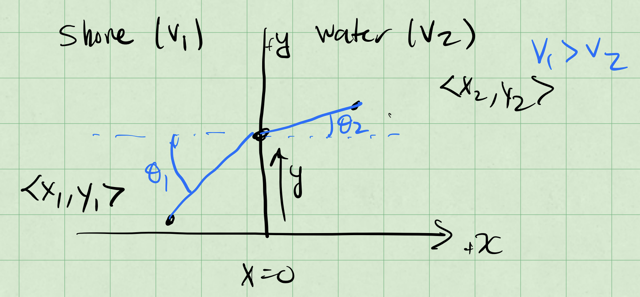
\includegraphics[keepaspectratio,alt={Snell's Law Diagram}]{/Users/caballero/repos/teaching/modern-classical-mechanics/images/notes/week11/snells_shore.png}}
\caption{Snell's Law Diagram}
\end{figure}

Notice the angle that we approach the shoreline at, \(\theta_1\), and
the angle that we approach the target in the water, \(\theta_2\).

The total time to travel from \(\langle x_1, y_1 \rangle\) to
\(\langle 0, y \rangle\) and then to \(\langle x_2, y_2 \rangle\) is:

\[T = t_1 + t_2 = \dfrac{d_1}{v_1} + \dfrac{d_2}{v_2}\]

where \(d_1\) is the distance from \(\langle x_1, y_1 \rangle\) to
\(\langle 0, y \rangle\), and \(d_2\) is the distance from
\(\langle 0, y \rangle\) to \(\langle x_2, y_2 \rangle\). We can write
those distances in terms of the coordinates:

\[d_1 = \sqrt{x_1^2 + (y - y_1)^2}\]
\[d_2 = \sqrt{x_2^2 + (y_2 - y)^2}\]

This gives us:

\[T = \dfrac{\sqrt{x_1^2 + (y - y_1)^2}}{v_1} + \dfrac{\sqrt{x_2^2 + (y_2 - y)^2}}{v_2}.\]

We want to minimize this time, \(T\), by choosing the optimal point
\(y\) where we cross the shoreline. We compute the derivative of \(T\)
with respect to \(y\) and set it to zero:

\[\dfrac{dT}{dy} = 0\]

\[\dfrac{dT}{dy} = \dfrac{1}{2}\dfrac{1}{v_1}\left(x_1^2 + (y-y_1)^2\right)^{-1/2}(2)(y-y_1) + \dfrac{1}{2}\dfrac{1}{v_2}\left(x_2^2 + (y_2-y)^2\right)^{-1/2}(-2)(y_2-y) = 0\]
\[\dfrac{dT}{dy} = \dfrac{1}{v_1}\left(\dfrac{y-y_1}{\sqrt{x_1^2 + (y-y_1)^2}}\right) - \dfrac{1}{v_2}\left(\dfrac{y_2-y}{\sqrt{x_2^2 + (y_2-y)^2}}\right) = 0\]
\[\dfrac{dT}{dy} = \dfrac{1}{v_1}\left(\dfrac{y-y_1}{d_1}\right) - \dfrac{1}{v_2}\left(\dfrac{y_2-y}{d_2}\right) = 0\]

where the last step is just substituting in the expressions for \(d_1\)
and \(d_2\). Notice that those expressions are related to the angles we
defined earlier. We can rewrite the expression in terms of the angles
\(\theta_1\) and \(\theta_2\):

\[\sin(\theta_1) = \frac{y - y_1}{d_1}\]
\[\sin(\theta_2) = \frac{y_2 - y}{d_2}\]

This gives us:

\[\dfrac{\sin(\theta_1)}{v_1} - \dfrac{\sin(\theta_2)}{v_2} = 0\]

```\{important\} This is
\href{https://en.wikipedia.org/wiki/Snell\%27s_law}{\textbf{Snell's
Law}}! It tells us that the ratio of the sine of the angles to the
velocities is constant. This is a classic result in optics, but it also
applies to this problem of finding the shortest path in a plane.

\[\dfrac{\sin(\theta_1)}{v_1} = \dfrac{\sin(\theta_2)}{v_2}\] ```

    \subsection{Example: Brachistochrone
Problem}\label{example-brachistochrone-problem}

The
\href{https://en.wikipedia.org/wiki/Brachistochrone_problem}{Brachistochrone
problem} is a classic problem in the Calculus of Variations. It asks the
question: ``What is the shape of the curve that a bead will follow under
the influence of gravity to reach the bottom in the shortest time?''
Here's a great video from
\href{https://en.wikipedia.org/wiki/Steven_Strogatz}{Steven Strogatz}
that explains the problem and its solution.

\href{https://www.youtube.com/watch?v=Cld0p3a43fU}{\pandocbounded{
\includegraphics[keepaspectratio,alt={Youtube Video on the Brachistochrone Problem}]{/Users/caballero/repos/teaching/modern-classical-mechanics/images/notes/week11/Cld0p3a43fU.jpg}}}

Source: \url{https://www.youtube.com/watch?v=Cld0p3a43fU}

The setup is below, there's two points separated by a distance
vertically and horizontally. What shape should we make a track so that a
bead will roll down it in the shortest time?

\begin{figure}
\centering
\pandocbounded{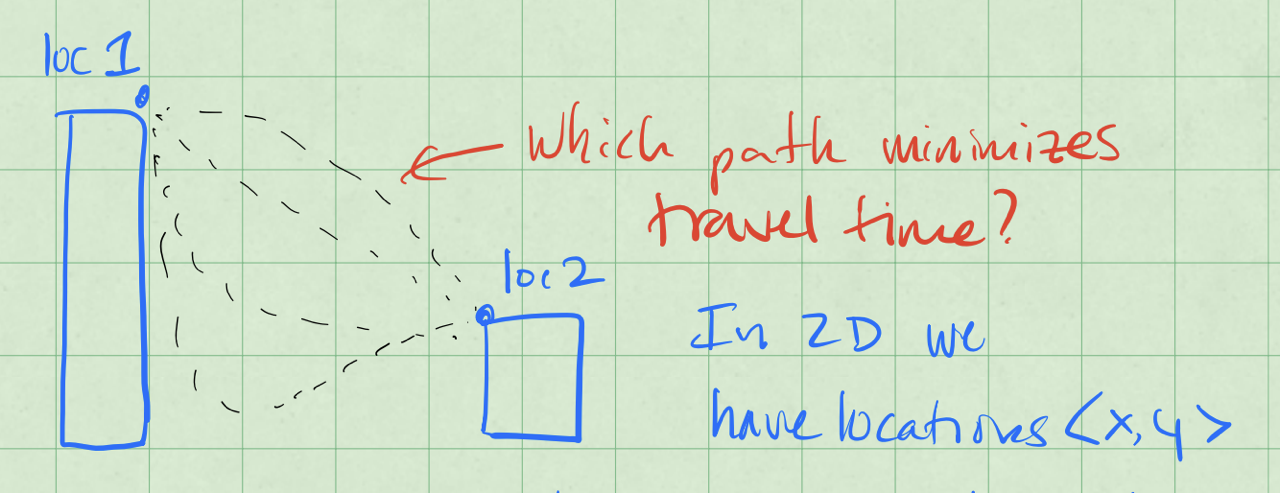
\includegraphics[keepaspectratio,alt={The Brachistochrone Problem}]{/Users/caballero/repos/teaching/modern-classical-mechanics/images/notes/week11/brachistochrone.png}}
\caption{The Brachistochrone Problem}
\end{figure}

    The time it takes for the bead to roll down the curve is given by:

\[T = \int_{1}^{2} \dfrac{ds}{v}\]

where \(ds\) is the differential arc length along the curve, and \(v\)
is the velocity of the bead at that point. The generic step is the same
as before:

\[ds = \sqrt{dx^2 + dy^2}.\]

\paragraph{Velocity of the Bead}\label{velocity-of-the-bead}

What about \(v\)? Because the bead is moving under the influence of
gravity, we can use conservation of energy to find the velocity. Note
that we don't model the rolling of the bead, just the motion down the
track. We also neglect all frictional forces. This is a major
simplification, but it will give us an analytical solution.

\[\Delta K + \Delta U = 0\]

If the bead starts from rest, then \(v_i = 0\), and we can write:

\[\dfrac{1}{2}mv^2 - \dfrac{1}{2}m(0)^2 + mg(\Delta y) = 0,\]

\[v = \sqrt{2g\Delta y}\]

where \(\Delta y = y_1 - y_2 > 0\). This is the change in height of the
bead as it rolls down the track. We can express this in terms of the
coordinates of the two points, \(y_1\) and \(y_2\).

Let's move the origin to the top of the track and measure \(+y\)
downwards. Thus, for any point on the track, we have:

\[v = \sqrt{2gy}.\]

We can now write the integral again,

\[T = \int_{1}^{2} \dfrac{ds}{v} = \int_{1}^{2} \dfrac{\sqrt{dx^2 + dy^2}}{\sqrt{2gy}}.\]

We notice that we can factor out a \(dy\) term from the square root in
the numerator:

\[\sqrt{dx^2 + dy^2} = dy\sqrt{\left(\frac{dx}{dy}\right)^2 + 1} = dy \sqrt{x'^2 + 1}\]

where \(x' = \frac{dx}{dy}\). This gives us:

\[T = \dfrac{1}{\sqrt{2g}}\int_{0}^{y_2} dy \dfrac{\sqrt{x'^2 + 1}}{\sqrt{y}}.\]

We can identify our function \(f\) as:

\[f(x,x',y) = f(x',y) = \dfrac{\sqrt{x'^2 + 1}}{\sqrt{y}}.\]

Because \(f\) does not depend on \(x\), \(\partial f/\partial x = 0\).
So that the Euler-Lagrange equation simplifies to:

\[\dfrac{d}{dy}\left(\dfrac{\partial f}{\partial x'}\right) = 0.\]

Or that this partial derivative must be a constant:

\[\dfrac{\partial f}{\partial x'} = \textrm{a constant},\]

\[\dfrac{\partial f}{\partial x'} = \dfrac{x'}{\sqrt{x'^2 + 1}\sqrt{y}} = \sqrt{C},\]

where \(C\) is a constant. We square both sides to get:

\[\dfrac{x'^2}{(x'^2 + 1)y} = C.\]

Knowing the solution ahead of time, we choose the constant
\(C = \frac{1}{2a}\). This gives us:

\[\dfrac{x'^2}{(x'^2 + 1)y} = \frac{1}{2a}.\]

Some more algebra gives us:

\[2ax'^2 = y(x'^2 + 1),\] \[(2a - y)x'^2 = y,\]
\[x'^2 = \frac{y}{2a - y},\]

where \(x' = \frac{dx}{dy}\). We can now integrate this to find the
shape of the curve:

\[x = \int \sqrt{\frac{y}{2a - y}} dy.\]

This integral will give us the shape of the curve \(x(y)\), but to solve
it we need to use a substitution.

Let \(y = a(1 - \cos(\theta))\). Thus, \(dy = a\sin(\theta)d\theta\).
This gives us:

\[x(y(\theta)) = \int \sqrt{\frac{y(\theta)}{2a - y(\theta)}} dy\]
\[x(y(\theta)) = \int \sqrt{\frac{a(1 - \cos(\theta))}{2a - a(1 - \cos(\theta))}} a\sin(\theta)d\theta\]
\[x(y(\theta)) = a \int \sqrt{\frac{(1-\cos\theta)}{(1+\cos\theta)}} \sin(\theta)d\theta.\]

Note that
\(\sin \theta = \sqrt{1 - \cos^2 \theta} = \sqrt{(1 - \cos\theta)(1 + \cos\theta)}\).
This allows us to simplify the integral:

\[x(y(\theta)) = a \int \sqrt{\frac{(1-\cos\theta)^2(1+\cos\theta)}{(1+\cos\theta)}} d\theta\]
\[x(y(\theta)) = a \int \sqrt{(1 - \cos\theta)^2} d\theta\]
\[x(y(\theta)) = a \int (1 - \cos\theta) d\theta\]
\[x(y(\theta)) = a \left(\theta - \sin(\theta)\right) + C\]

where \(C\) is a constant of integration.

With initial conditions \(x(0) = 0\) when \(y(0) = 0\) at \(t=0\) and
\(\theta = 0\), we find that \(C = 0\). So the solution is:

\[x(\theta) = a\left(\theta - \sin(\theta)\right)\]
\[y(\theta) = a(1 - \cos(\theta)).\]

This is the ``cycloid'' curve that the bead will follow to minimize the
time it takes to roll down the track. We can plot this curve to
visualize it.

What is so interesting about this curve is that it is
\href{https://en.wikipedia.org/wiki/Isochronous}{isochronous}, meaning
that all beads released from rest at any point on the curve will reach
the bottom at the same time, regardless of where they start.

    \begin{tcolorbox}[breakable, size=fbox, boxrule=1pt, pad at break*=1mm,colback=cellbackground, colframe=cellborder]
\prompt{In}{incolor}{27}{\boxspacing}
\begin{Verbatim}[commandchars=\\\{\}]
\PY{c+c1}{\PYZsh{}\PYZsh{} Plot a cycloid path for comparison}
\PY{c+c1}{\PYZsh{}\PYZsh{} \PYZdl{}\PYZdl{}x(\PYZbs{}theta) = a\PYZbs{}left(\PYZbs{}theta \PYZhy{} \PYZbs{}sin(\PYZbs{}theta)\PYZbs{}right)\PYZdl{}\PYZdl{}}
\PY{c+c1}{\PYZsh{}\PYZsh{} \PYZdl{}\PYZdl{}y(\PYZbs{}theta) = a(1 \PYZhy{} \PYZbs{}cos(\PYZbs{}theta)).\PYZdl{}\PYZdl{}}

\PY{k+kn}{import}\PY{+w}{ }\PY{n+nn}{numpy}\PY{+w}{ }\PY{k}{as}\PY{+w}{ }\PY{n+nn}{np}
\PY{k+kn}{import}\PY{+w}{ }\PY{n+nn}{matplotlib}\PY{n+nn}{.}\PY{n+nn}{pyplot}\PY{+w}{ }\PY{k}{as}\PY{+w}{ }\PY{n+nn}{plt}
\PY{n}{plt}\PY{o}{.}\PY{n}{style}\PY{o}{.}\PY{n}{use}\PY{p}{(}\PY{l+s+s1}{\PYZsq{}}\PY{l+s+s1}{seaborn\PYZhy{}v0\PYZus{}8\PYZhy{}colorblind}\PY{l+s+s1}{\PYZsq{}}\PY{p}{)}

\PY{c+c1}{\PYZsh{} Cycloid parameters}
\PY{n}{a} \PY{o}{=} \PY{l+m+mi}{1}  \PY{c+c1}{\PYZsh{} Radius of the rolling circle}
\PY{n}{theta} \PY{o}{=} \PY{n}{np}\PY{o}{.}\PY{n}{linspace}\PY{p}{(}\PY{l+m+mi}{0}\PY{p}{,} \PY{l+m+mi}{3}\PY{o}{/}\PY{l+m+mi}{2} \PY{o}{*} \PY{n}{np}\PY{o}{.}\PY{n}{pi}\PY{p}{,} \PY{l+m+mi}{1000}\PY{p}{)}  \PY{c+c1}{\PYZsh{} Parameter for the cycloid}

\PY{c+c1}{\PYZsh{} Cycloid equations}
\PY{n}{x\PYZus{}cycloid} \PY{o}{=} \PY{n}{a} \PY{o}{*} \PY{p}{(}\PY{n}{theta} \PY{o}{\PYZhy{}} \PY{n}{np}\PY{o}{.}\PY{n}{sin}\PY{p}{(}\PY{n}{theta}\PY{p}{)}\PY{p}{)}
\PY{n}{y\PYZus{}cycloid} \PY{o}{=} \PY{o}{\PYZhy{}}\PY{n}{a} \PY{o}{*} \PY{p}{(}\PY{l+m+mi}{1} \PY{o}{\PYZhy{}} \PY{n}{np}\PY{o}{.}\PY{n}{cos}\PY{p}{(}\PY{n}{theta}\PY{p}{)}\PY{p}{)}

\PY{c+c1}{\PYZsh{} Create the plot}
\PY{n}{fig}\PY{p}{,} \PY{n}{ax} \PY{o}{=} \PY{n}{plt}\PY{o}{.}\PY{n}{subplots}\PY{p}{(}\PY{n}{figsize}\PY{o}{=}\PY{p}{(}\PY{l+m+mi}{10}\PY{p}{,} \PY{l+m+mi}{4}\PY{p}{)}\PY{p}{)}  \PY{c+c1}{\PYZsh{} Create a new figure and axis}
\PY{n}{ax}\PY{o}{.}\PY{n}{plot}\PY{p}{(}\PY{n}{x\PYZus{}cycloid}\PY{p}{,} \PY{n}{y\PYZus{}cycloid}\PY{p}{,} \PY{n}{color}\PY{o}{=}\PY{l+s+s1}{\PYZsq{}}\PY{l+s+s1}{C0}\PY{l+s+s1}{\PYZsq{}}\PY{p}{)}
\PY{n}{ax}\PY{o}{.}\PY{n}{plot}\PY{p}{(}\PY{l+m+mi}{0}\PY{p}{,} \PY{l+m+mi}{0}\PY{p}{,} \PY{l+s+s1}{\PYZsq{}}\PY{l+s+s1}{C1o}\PY{l+s+s1}{\PYZsq{}}\PY{p}{,} \PY{n}{label}\PY{o}{=}\PY{l+s+s1}{\PYZsq{}}\PY{l+s+s1}{Start}\PY{l+s+s1}{\PYZsq{}}\PY{p}{)}  \PY{c+c1}{\PYZsh{} Starting point of the cycloid}
\PY{n}{ax}\PY{o}{.}\PY{n}{plot}\PY{p}{(}\PY{n}{x\PYZus{}cycloid}\PY{p}{[}\PY{o}{\PYZhy{}}\PY{l+m+mi}{1}\PY{p}{]}\PY{p}{,} \PY{n}{y\PYZus{}cycloid}\PY{p}{[}\PY{o}{\PYZhy{}}\PY{l+m+mi}{1}\PY{p}{]}\PY{p}{,} \PY{l+s+s1}{\PYZsq{}}\PY{l+s+s1}{C2o}\PY{l+s+s1}{\PYZsq{}}\PY{p}{,} \PY{n}{label}\PY{o}{=}\PY{l+s+s1}{\PYZsq{}}\PY{l+s+s1}{End}\PY{l+s+s1}{\PYZsq{}}\PY{p}{)}  \PY{c+c1}{\PYZsh{} Ending point of the cycloid}

\PY{c+c1}{\PYZsh{} Set labels and title}
\PY{n}{ax}\PY{o}{.}\PY{n}{set\PYZus{}xlabel}\PY{p}{(}\PY{l+s+s1}{\PYZsq{}}\PY{l+s+s1}{x}\PY{l+s+s1}{\PYZsq{}}\PY{p}{)}
\PY{n}{ax}\PY{o}{.}\PY{n}{set\PYZus{}ylabel}\PY{p}{(}\PY{l+s+s1}{\PYZsq{}}\PY{l+s+s1}{y}\PY{l+s+s1}{\PYZsq{}}\PY{p}{)}
\PY{n}{ax}\PY{o}{.}\PY{n}{set\PYZus{}title}\PY{p}{(}\PY{l+s+s1}{\PYZsq{}}\PY{l+s+s1}{Cycloid Path}\PY{l+s+s1}{\PYZsq{}}\PY{p}{)}

\PY{n}{ax}\PY{o}{.}\PY{n}{legend}\PY{p}{(}\PY{p}{)}  \PY{c+c1}{\PYZsh{} Add a legend to the plot}

\PY{c+c1}{\PYZsh{} Show the plot}
\PY{n}{plt}\PY{o}{.}\PY{n}{grid}\PY{p}{(}\PY{k+kc}{True}\PY{p}{)}  \PY{c+c1}{\PYZsh{} Add grid for better readability}
\PY{n}{plt}\PY{o}{.}\PY{n}{show}\PY{p}{(}\PY{p}{)}  \PY{c+c1}{\PYZsh{} Display the plot}
\end{Verbatim}
\end{tcolorbox}

    \begin{center}
    \adjustimage{max size={0.9\linewidth}{0.9\paperheight}}{11_notes_files/11_notes_10_0.png}
    \end{center}
    { \hspace*{\fill} \\}
    
    


    % Add a bibliography block to the postdoc
    
    
    
\end{document}
